%HOMEWORK template for M 325K
\documentclass{beamer}
\usetheme{Antibes}



%Begin package import

\usepackage{amsmath, amssymb, amsthm}
\usepackage{mathtools}
\usepackage{pdfpages}
\usepackage{tikz-cd}
\usepackage{mathabx}
\usepackage{amsmath}


%End package import
%Begin custom commands

\newcommand{\C}{\mathbb{C}}
\newcommand{\h}[1]{\hat{#1}}
\newcommand{\R}{\mathbb{R}}
\newcommand{\Q}{\mathbb{Q}}
\newcommand{\Z}{\mathbb{Z}}
\newcommand{\N}{\mathbb{N}}
\newcommand{\F}{\mathcal{F}}
\newcommand{\aabs}[1]{\left\lvert\left\lvert #1\right\rvert\right\rvert}

\newcommand{\abs}[1]{\left\lvert #1\right\rvert}
\newcommand{\RM}[1]{\mathrm{#1}}
\newcommand{\BF}[1]{\textbf{#1}}
\newcommand{\e}{\epsilon}
\newcommand{\ceil}[1]{\lceil{#1}\rceil}
\newcommand{\floor}[1]{\lfloor{#1}\rfloor}
\newcommand{\rarr}[0]{\rightarrow}
\newcommand{\IM}[1]{\text{Im}(#1)}
\newcommand{\Hom}[0]{\text{Hom}}
\newcommand{\Pow}[1]{\text{Pow}(#1)}
\newcommand{\angles}[1]{\langle #1 \rangle}

%End custom commands
%Begin custom theorems

\newtheorem{innercustomgeneric}{\customgenericname}
\providecommand{\customgenericname}{}
\newcommand{\newcustomtheorem}[2]{%
\newenvironment{#1}[1]
{%
\renewcommand\customgenericname{#2}%
\renewcommand\theinnercustomgeneric{##1}%
\innercustomgeneric%
}
{\endinnercustomgeneric}
}




%Information to be included in the title page:
\title{Managing Variance: Heisenberg-Weyl Inequality}
\author{Arham Rajendra Lodha}
\institute{University of Texas at Austin}
\date{Summer 2024}

\begin{document}

\frame{\titlepage}

\begin{frame}
    \frametitle{Table of Contents}
    \tableofcontents
\end{frame}

\section{Motivation}
\begin{frame}
    \frametitle{Motivation}

    Some of the main ideas in elementary harmonic analysis are related to understanding the duality between a function and its fourier transform. The Heisenberg-Weyl Inequality is one such duality relating the spread of a function in $L^2(\R)$ with the spread of its fourier transform.      
    
\end{frame}

\section{Definitions and Basic Concepts}
\subsection{Understanding $L^2(\R)$ }
\begin{frame}
    \frametitle{Understanding $L^2(\R)$ }

    \begin{block}{Definition}
        $\mathbf{L^2(\R)}$ is the space of functions $f: \R \to \C$ such that
        
        \[
            \abs{\abs{f}}_{L^2} := \sqrt{\int_{-\infty}^{\infty} |f(x)|^2 dx} < \infty 
        \]

        \pause

        $\mathbf{L^2(\R)}$ also has a natural inner product defined as follows $\forall f, g \in L^2(\R)$, \[\angles{f, g} = \int_{\infty}^{\infty} f(x) \overline{g(x)} dx\]
        
        Note $\aabs{f}_{L^2}^2 = \angles{f, f}$ and $L^2(\R)$ is a Hilbert space with respect to this norm and inner product.   
    \end{block}
\end{frame}



\subsection{Fourier Transform}
\begin{frame}
    \frametitle{The Fourier Transform}


    \begin{definition}
        Let $e_n(x) := e^{2 \pi i n x}$.
        $\forall f \in L^2(\R)$, let $\h{f} : \R \to \C$ where $\forall n \in \R$, 
        
        \[\h{f}(n) = \angles{f, e_n} = \int_{-\infty}^{\infty}f(x) e^{-2 \pi i n x} dx\] 
        
        and 

        \[
        f(x) = \int_{-\infty}^{\infty}\h{f}(n) e^{2 \pi i x n} dn. 
        \]

        Let $\mathcal{F}$ be the Fourier Transform which takes $f \to \h{f}$.   
    \end{definition}
    

\end{frame}

\begin{frame}
    \frametitle{Inverse Fourier Transform}


    \begin{block}{Definition}
        $\forall f \in L^2(\R)$, there also exists a inverse transform $\mathcal{F}^{-1}$ which takes $\h{f} \to f$ \[
        \mathcal{F}^{-1}[\h{f}](x) = \angles{\h{f}, e_{-x}}= \int_{-\infty}^{\infty} \h{f}(n) e^{2 \pi i x n} dn
        \] 
    \end{block}

\end{frame}

\begin{frame}
    \frametitle{$C_{\downarrow}^{\infty}(\R)$ as a subset of $L^2(\R)$ }

    \begin{block}{Remark}
        $C_{\downarrow}^{\infty}(\R)$ is the set of infinitely differentiable rapidly decreasing functions on $\R$. Infinitely differentiable means that $f \in \C^{\infty}(R)$ and "rapidly decreasing" applies to $f, f', f'', \dots$, and means that \[
        x^p \frac{d^q f}{dx^q} \to 0 \text{ as } \abs{x} \to \infty 
        \]
        
        for every nonnegative integral $p$ and $q$.   
    \end{block}

    \pause

    \begin{block}{Important Fact!}
        $C_{\downarrow}^{\infty}(\R)$ is a dense subset of $L^{2}(\R)$. Most proofs regarding properties of $L^2(\R)$ use this fact.    
    \end{block}
\end{frame}

\begin{frame}
    \frametitle{The Fourier Transform is a isomorphism of $L^2(\R)$ }

    \begin{theorem}
        $\mathcal{F}$ is a isomorphism of $L^2(\R)$ and $\mathcal{F}^{-1}$ is actually its inverse function.    
    \end{theorem}
    \pause
    \begin{block}{Corollary: Plancherel Identity}
        $\forall f \in L^2(\R)$, \[\abs{\abs{f}}_{L^2} = ||\h{f}||_{L^2}\] 
    \end{block}
    \pause
    \begin{block}{Corollary: Parseval's Identity}
        $\forall f, g \in L^2(\R)$, \[\angles{f, g} = \angles{\h{f}, \h{g}}\]  
    \end{block}
\end{frame}

\begin{frame}
    \frametitle{Major Identities (Cont.)}

    \begin{block}{Theorem: Effect of Differentiation}
        $\forall f \in L^2(\R)$, $            \h{f'}(n) = 2 \pi i n \h{f}(x)
$.   
    \end{block}

    \pause

    \begin{block}{Theorem: Effect of Translation}
        $\forall f \in L^2(\R)$ and $\forall h \in \R$, let $f_h(x) = f(x - h)$. \[\h{f_h}(n) = e^{-2 \pi i n h} \h{f}(n)\]. 
    \end{block}

    \pause

    \begin{block}{Theorem: Effect of Scaling}
        $\forall f \in L^2(\R)$ and $\forall h \in \R$, $f_h(x) = hf(x)$, \[\h{f_h}(n) = \h{f}(n / h)\]
    \end{block}

\end{frame}

\section{Proving The Heisenberg-Weyl Inequality}
\subsection{Defining Things}
\begin{frame}
    \frametitle{Measure of Variance}

    \begin{definition}
        $\forall f \in L^2(\R)$, let \[t_0 = \mathbb{E}_f[X] = \int_{-\infty}^{\infty}x f(x) dx.\] 
        
        Define $\sigma^2(f) := \abs{\abs{(x - t_0)f}}_{L^2}^2$ be the variance of a function.  
    \end{definition}

\end{frame}

\subsection{Lets start proving!}
\begin{frame}
    \frametitle{The Heisenberg-Weyl Inequality}

    \begin{block}{Theorem: The Heisenberg-Weyl Inequality}
        $\forall f \in L^2(\R)$, 
        
        \[
            \sigma^2(f)\sigma^2(\h{f}) \geq \frac{\aabs{f}_{L^2}^4}{16 \pi^2}
        \],

        with equality \textbf{if and only if} f is a constant multiple of the gaussian, $e^{-kx^2}$ for $k > 0$.    
    \end{block}

\end{frame}

\subsection{Simplifying assumptions}

\begin{frame}
    \frametitle{The Proof}

    For all $f \in L^2(\R)$, let $t_0 = \mathbb{E}_f[X]$. Let $F(x) := f(x + t_0)$. Thus $\mathbb{E}_{F}[X] = 0$. So
        
    \[\sigma^2(f) = \int_{-\infty}^{\infty}(x - t_0)^2 \abs{f(x)}^2 dx = \int_{-\infty}^{\infty}x^2 \abs{f(x + t_0)}^2 dx = \sigma^2(F). \]

    Thus without a loss of generality, we can assume the center of mass of $f$ is 0 for the rest of the proof.  

\end{frame}

\begin{frame}
    \frametitle{The Proof}

    Because $\sigma^2(f) = \aabs{xf}_{L^2}^2 > 0$, we may as well suppose $\sigma^2(\h{f}) = \aabs{n\h{f}}_{L^2}^2 < \infty$ because otherwise there is nothing to prove. Thus 
        
        \begin{align*}
            n\h{f} \in L^2(\R) &\implies 2 \pi i n \h{f} = \h{f'} \in L^2(\R) & \text{(Effect of Differentiation)}\\
            &\implies \F^{-1}[\h{f'}] = f' \in L^2(\R)
        \end{align*}

\end{frame}

\subsection{Working with Inequalities}

\begin{frame}
    \frametitle{The Proof}

    \begin{align*}
        4 \pi^2 \sigma^2(f) \sigma^2(\h{f}) &= 4 \pi^2 \int_{-\infty}^{\infty} \abs{xf(x)}^2 dx \int_{-\infty}^{\infty} \abs{n \h{f}(n)}^2 d n \\
        &= \int_{-\infty}^{\infty} \abs{xf(x)}^2 dx \int_{-\infty}^{\infty} \abs{2 \pi i n \h{f}(n)}^2 d n \\
        &= \int_{-\infty}^{\infty} \abs{xf(x)}^2 dx \int_{-\infty}^{\infty} \abs{\h{f'}(n)}^2 d n. 
    \end{align*}

    The last equality is true by the \textbf{Effect of Differentiation}. 

\end{frame}

\begin{frame}
    \frametitle{The Proof}

    \begin{align*}
        4 \pi^2 \sigma^2(f) \sigma^2(\h{f}) &= \int_{-\infty}^{\infty} \abs{xf(x)}^2 dx \int_{-\infty}^{\infty} \abs{\h{f'}(n)}^2 d n \\
        &= \int_{-\infty}^{\infty} \abs{xf(x)}^2 dx \aabs{\h{f'}}_{L^2}^2 \\
        &= \int_{-\infty}^{\infty} \abs{xf(x)}^2 dx \aabs{f'}_{L^2}^2 \textbf{(Plancheral Identity)} \\
        &= \angles{xf, xf} \angles{f', f'} = \angles{\abs{xf}, \abs{xf}} \angles{\abs{f'}, \abs{f'}}\\ &= \angles{\abs{xf}, \abs{xf}}\angles{\abs{\overline{f'}}, \abs{\overline{f'}}} \\
        &\geq \abs{\angles{\abs{f'}, \abs{xf}}}^2 \textbf{ (Cauchy Shwartz Inequality)} \\
        &= \angles{\abs{f'}, \abs{xf}}^2
    \end{align*}


\end{frame}

\begin{frame}
    \frametitle{The Proof}

    \begin{align*}
        4 \pi^2 \sigma^2(f) \sigma^2(\h{f}) &\geq \angles{\abs{f'}, \abs{xf}}^2 \\
        &= \left[\int_{-\infty}^{\infty} \abs{xf'(x)\overline{f(x)}}  dx\right]^2 \\
        &\geq \left[\int_{-\infty}^{\infty}\Re[xf'(x)\overline{f(x)}]  dx\right]^2 \\
        &= \left[\int_{-\infty}^{\infty} \frac{1}{2}(xf'(x)\overline{f(x)} + \overline{xf'(x)\overline{f(x)}})dx\right]^2 \\ 
        &= \frac{1}{4} \left[\int_{-\infty}^{\infty} x(f'(x)\overline{f(x)} + \overline{f'(x)}f(x))dx\right]^2
    \end{align*}

\end{frame}

\subsection{Bringing In $C^{\infty}_{\downarrow}(\R)$ }

\begin{frame}
    \frametitle{The Proof}

    We are now stuck at this integral, to get a value for the integral create a sequence $f_n \in C^{\infty}_{\downarrow}(\R)$ such that $f_n \to f$ and 

    \[
    \lim_{n \to \infty}\int_{-\infty}^{\infty}(1 + 4 \pi^2 n^2) \abs{\h{f_n}(n) - \h{f}(n)}^2 d n = 0. 
    \]

    This condition on convergence leads to the fact that $f_n$ converges to $f$ pointwise modulo some technical flourishes.   
\end{frame}


\begin{frame}
    \frametitle{The Proof}

    \begin{lemma}
        $\forall f \in C^1(\R)$, $\frac{d}{dx} \abs{f(x)}^2 = \frac{d}{dx}(f(x)\overline{f(x)}) = f'(x)\overline{f(x)} + f(x)\overline{f'(x)}$ 
    \end{lemma}

    \begin{lemma}
        $\forall f \in L^2(\R)$, $\abs{f(x)} \in L^2(\R)$ because \[
            \aabs{\abs{f}}_{L^2}^2 = \int_{-\infty}^{\infty} \abs{\abs{f(x)}}^2 dx = \int_{-\infty}^{\infty} \abs{f(x)}^2dx = \aabs{f}_{L^2}^2
        \]   
    \end{lemma}


\end{frame}

\begin{frame}
    \frametitle{The Proof}

    \begin{align*}
        &\int_{-\infty}^{\infty} x(f'(x)\overline{f(x)} + \overline{f'(x)}f(x))dx \\=& \lim_{m \to \infty} \lim_{n \to \infty} \int_{-m}^{m} x(f_n'(x)\overline{f_n(x)} + \overline{f_n'(x)}f_n(x))dx \\
        =& \lim_{m \to \infty} \lim_{n \to \infty} \int_{-m}^{m} x \frac{d}{dx}\abs{f_n(x)}^2 dx\\
        =& \lim_{m \to \infty} \lim_{n \to \infty} 
        \left([x\abs{f_n(x)}^2]^{m}_m - \int_{-m}^{m}\abs{f_n(x)}^2 dx \right)
    \end{align*} 

\end{frame}

\begin{frame}
    \frametitle{The Proof}

    \begin{align*}
        &\int_{-\infty}^{\infty} x(f'(x)\overline{f(x)} + \overline{f'(x)}f(x))dx \\=& \lim_{m \to \infty} \lim_{n \to \infty} 
        \left([x\abs{f_n(x)}^2]^{m}_m - \int_{-m}^{m}\abs{f_n(x)}^2 dx \right) \\
        =&  \lim_{m \to \infty}(m(\abs{f(m)} + \abs{f(-m)})) - \aabs{f}_{L^2}^2 = - \aabs{f}_{L^2}^2
    \end{align*}

    $\lim_{m \to \infty}(m(\abs{f(m)}+ \abs{f(-m)})) = 0$ because otherwise $\abs{f(x)}^2 + \abs{f(-x)}^2$ would not be in $L^2(\R)$.   

\end{frame}

\begin{frame}
    \frametitle{The Proof}

    Thus, 

    \begin{align*}
        4 \pi^2 \sigma^2(f) \sigma^2(\h{f}) &\geq \frac{1}{4} \left[\int_{-\infty}^{\infty} x(f'(x)\overline{f(x)} + \overline{f'(x)}f(x))dx\right]^2 \\
        &= \frac{1}{4} \aabs{f}_{L^2}^4. 
    \end{align*}

    Finally, 

    \[
        \sigma^2(f) \sigma^2(\h{f}) \geq \frac{1}{16 \pi^2} \aabs{f}_{L^2}^4
    \]

\end{frame}

\begin{frame}
    \frametitle{The Proof}

    To get the lower bound, we look all the way back to the key application of the Cauchy Shwartz Inequality where $\angles{xf, xf}\angles{f', f'} \geq \abs{\angles{f', xf}}^2$ with equality if and only if $f' = kxf$ almost everywhere where $k \in \C$. 

\end{frame}

\begin{frame}
    \frametitle{The Proof}

    The second inequality was the fact that $|xf'\overline{f}|  \geq \Re(xf'\overline{f})$.  Lets use this condition to deduce a bit more about $k$.
    \[
       \abs{kx^2 \abs{f}} = \abs{kx^2 f \overline{f}} = |xf'\overline{f}| \geq \Re(xf'\overline{f}) = \Re(k x^2 f \overline{f}) = \Re(kx^2 \abs{f})
    \]

    This means $\abs{kx^2 \abs{f}} \geq \Re(kx^2 \abs{f})$. Equality is only possible if $kx^2 \abs{f} \in \R$ and $kx^2 \abs{f} \geq 0$ for all $x \in \R$. But since $x^2$ and $\abs{f}$ are in $\R$ and are greater than or equal to 0. That means $k \in \R$ and $k \geq 0$. But $k \neq 0$, because otherwise $f$ is a constant function and constant functions are not in $L^2(\R)$. Thus $f$ is a solution differential equation $f' = kxf$ for $k > 0$.  Thus $f$ is a multiple of the gaussian, $e^{-kx^2}$ for $k > 0$.                   

\end{frame}

\section{What does the Inequality Mean?}

\begin{frame}
    \frametitle{The Heisenberg-Weyl Inequality}

    \begin{block}{Theorem: The Heisenberg-Weyl Inequality}
        $\forall f \in L^2(\R)$, 
        
        \[
            \sigma^2(f)\sigma^2(\h{f}) \geq \frac{\aabs{f}_{L^2}^4}{16 \pi^2}
        \],

        with equality \textbf{if and only if} f is a constant multiple of the gaussian, $e^{-kx^2}$ for $k > 0$.    
    \end{block}

\end{frame}


\begin{frame}
    \frametitle{What does the inequality tell us?}
    
    \begin{figure}
        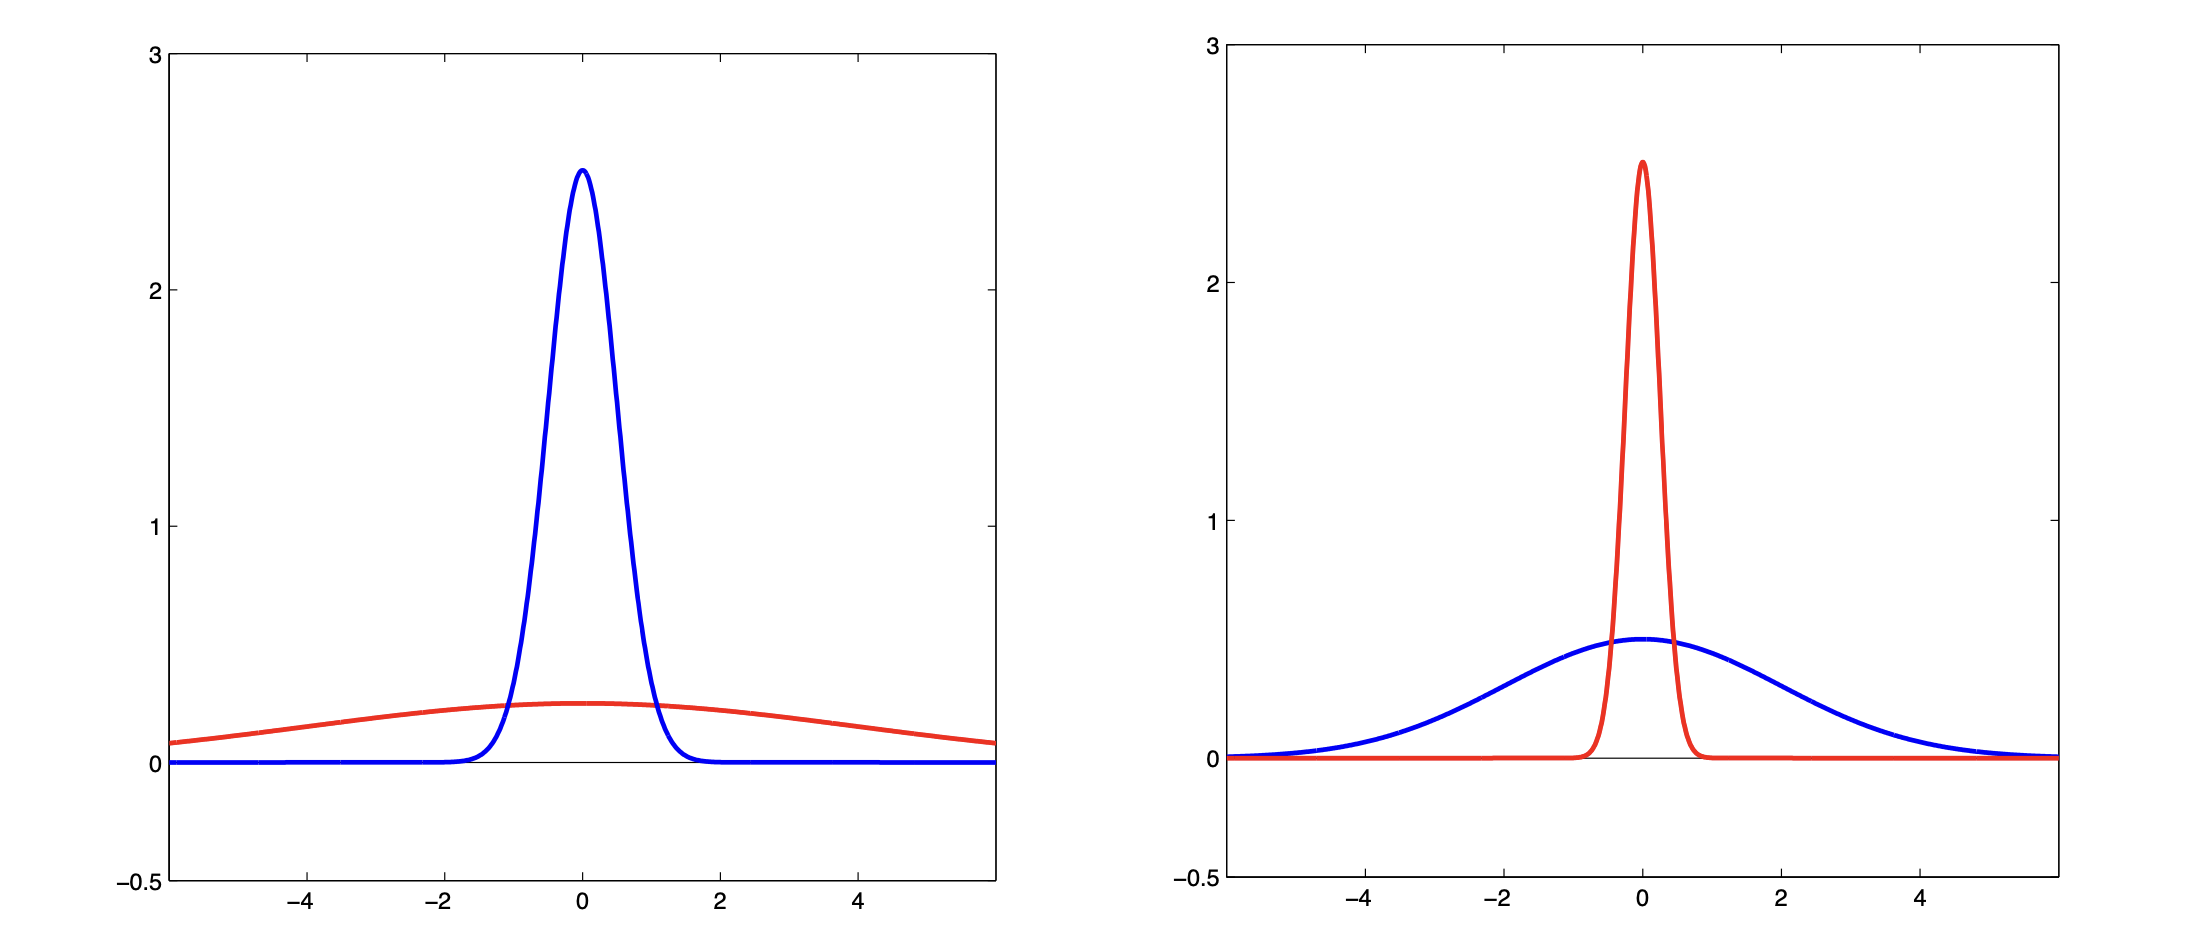
\includegraphics[scale=.30]{Picture.png}
    \end{figure}
\end{frame}

\begin{frame}
    \frametitle{The Heisenberg-Weyl Inequality}

    \begin{block}{Theorem: The Heisenberg Uncertainty Principle}
        Let $\psi$ be a wave function such that \[
            \int_{-\infty}^{\infty}\abs{\psi(x)}^2 dx= 1,
        \]      
        
        Let $A$ be the position operator and let $B$ be the momentum operator, such that $Af(x) = xf(x)$ and $Bf(x) = \frac{1}{2 \pi i}f'(x)$. 
        
        The Heisenberg-Weyl Inequality tells us, 

        \[
        Var(A)Var(B) \geq C 
        \] 

        for some fixed constant $C$.  
    \end{block}

\end{frame}



\end{document}
